\title{INTD262: Science or Not Science?}
\author{Dr. Jordan Hanson - Whittier College Dept. of Physics and Astronomy}
\date{\today}
\documentclass[12pt]{article}
\usepackage[margin=1.5cm]{geometry}
\usepackage{hyperref}
\usepackage{graphicx}
\usepackage{amsmath}
\begin{document}
\maketitle

\section{Introduction}

In this activity, we will attempt to classify fields of knowledge scientifically.  Recall that in the introduction and chapter 1 of \textit{The Scientific Attitude}, we find a discussion about the difference between subjects that are \textit{scientific}, and \textit{non-scientific}.  The \textit{non-scientific} category may be split into two categories.  The first sub-category of \textit{non-scientific} fields is comprised of subjects that are not meant to be forms of scientific inquiry (literature, history, languages).  The second sub-category of \textit{non-scientific} fields are those that \textit{impersonate} science: the \textit{pseudo-scientific} fields.  Examples of pseudo-science include astrology, creationism, and the link between vaccines and autism.  In this activity, we will example synopses of fields of study, and attempt to classify the relative scientific merit of the fields.  The goal of this activity is to understand that scientific thought exists along spectra of understanding.  Some fields are theoretically warranted, some are backed by voluminous empirical evidence, some have both, and some have neither.  Some fields make testable, falsifiable claims, while others do not.

\section{First Classification: Science vs. Non-Science}

\begin{figure}[ht]
\centering
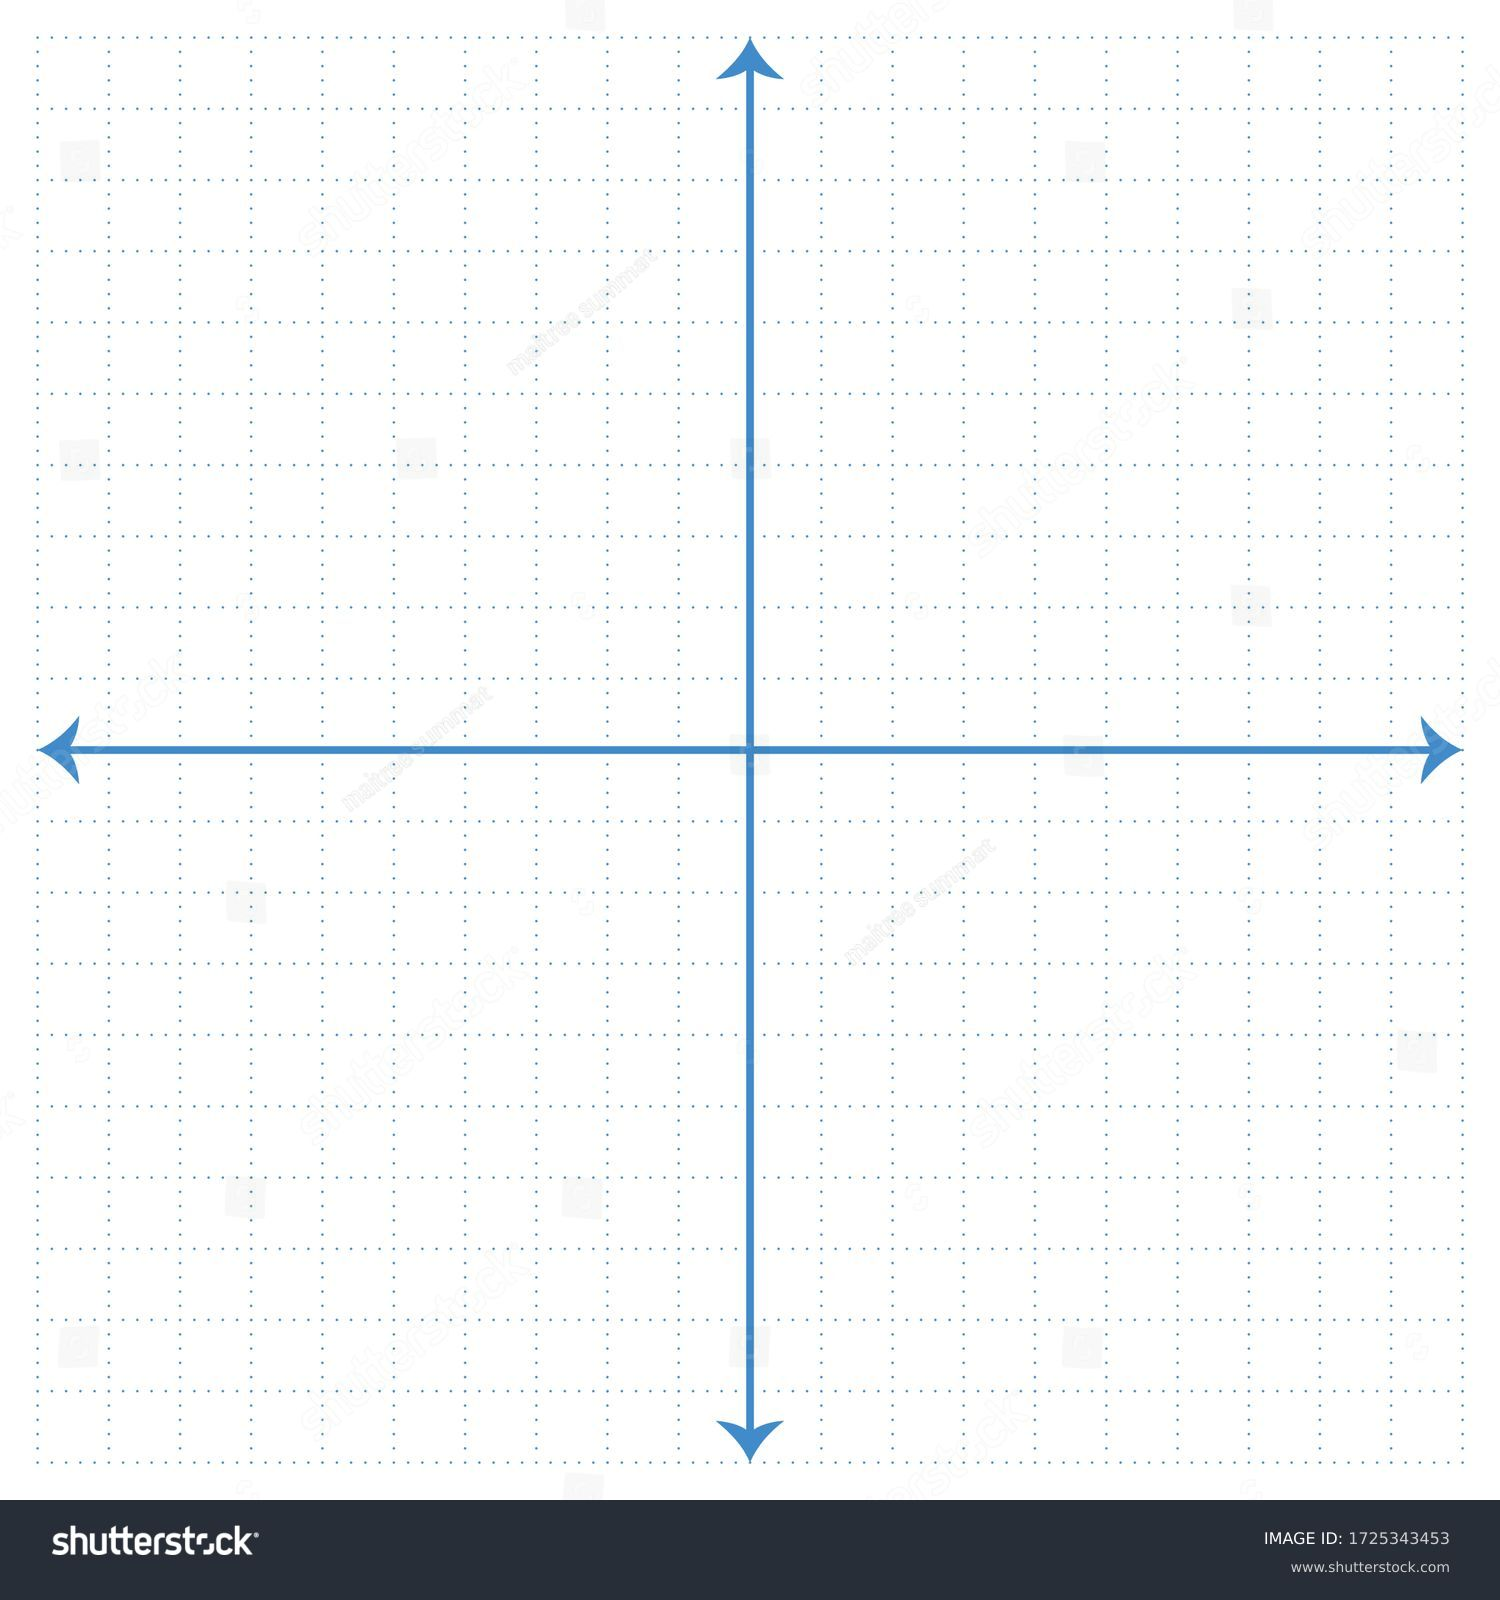
\includegraphics[width=0.45\textwidth,trim=0cm 3.5cm 0cm 0cm,clip=true]{figures/graph.jpg}
\caption{\label{fig:1} (a) On the right-hand side of the 2D graph above, label the axis ``testable.''  (b) On the top side of the 2D graph above, label the axis ``falsifiable.''}
\end{figure}

\clearpage

\section{Second Classification: Science vs. Pseudo-Science}

\begin{figure}[hb]
\centering
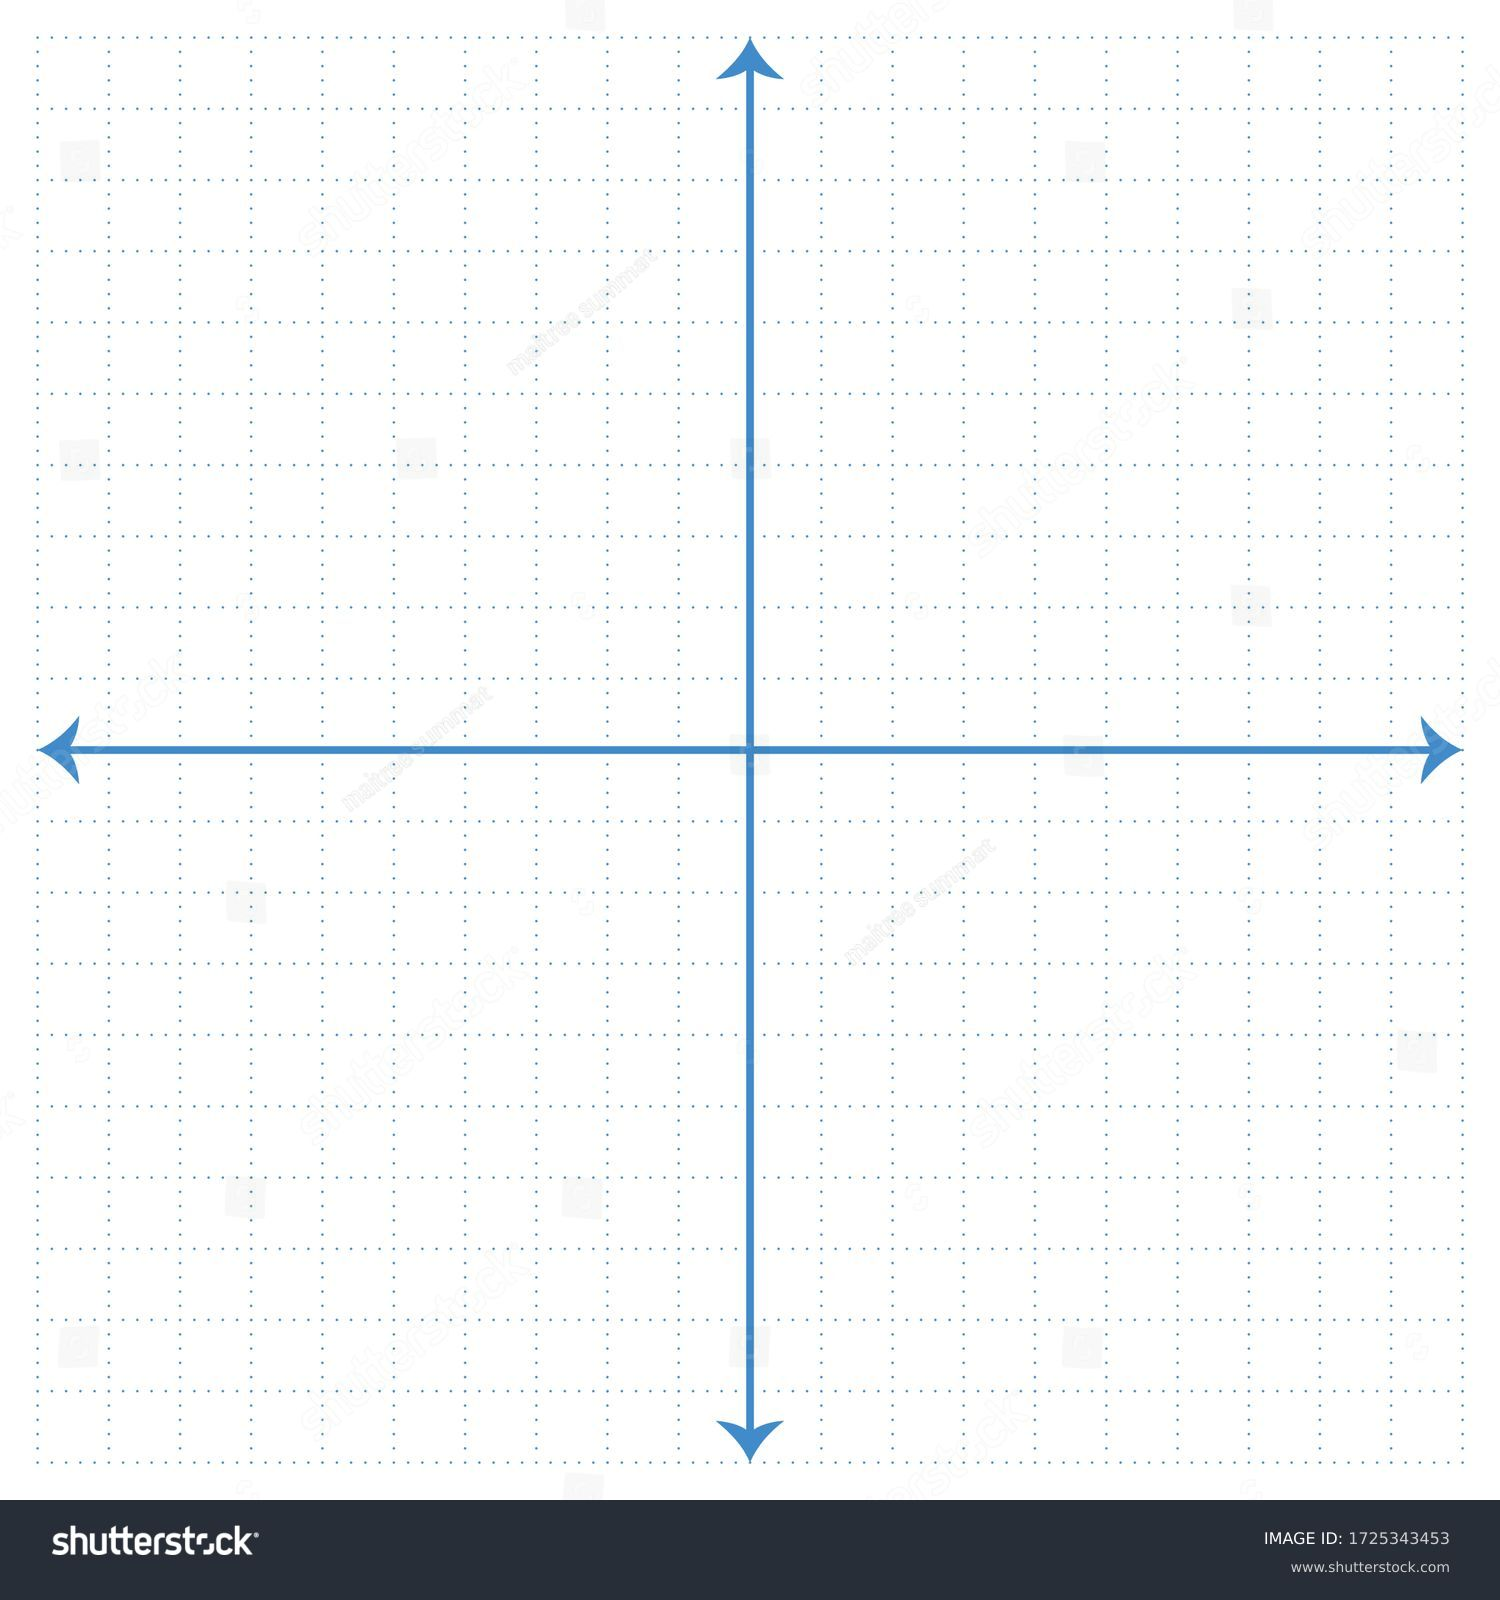
\includegraphics[width=0.45\textwidth,trim=0cm 3.5cm 0cm 0cm,clip=true]{figures/graph.jpg}
\caption{\label{fig:2}}
\end{figure}

\end{document}
